\documentclass{beamer}
\usepackage{xcolor}
\usepackage{mathtools}
\usetheme[titlepagelogo=firenze,% Logo for the first page
		  language=italian,
		  bullet=circle,
		  color=blue,
         ]{TorinoTh}
\usepackage[beamer,customcolors]{hf-tikz}
\usepackage[noend]{algpseudocode}
\usepackage[Algoritmo]{algorithm}
\renewcommand{\thealgorithm}{}
\definecolor{UniBlue}{RGB}{83,121,170}
\uselanguage{italian}
\languagepath{italian}
\deftranslation[to=italian]{Definition}{Definizione}
\deftranslation[to=italian]{Theorem}{Teorema}
\setbeamercolor{block title}{use=structure,fg=white,bg=UniBlue}
\setbeamercolor{block body}{use=structure,fg=black,bg=white}
\usepackage{proof}

\newcommand*{\bfrac}[2]{\genfrac{}{}{0pt}{1}{#1}{#2}}

\author{}
\rel{{\normalsize \emph{Elaborazione e Protezione delle Immagini}}\\\vspace{0.3cm}Lorenzo Cioni e Saverio Meucci}
\title{\huge Clustering di immagini basato su Normalized Cuts per l’identificazione di camera}
\date{28 Giugno 2016}

\begin{document}

\titlepageframe

%-- Introduzione --%

\begin{tframe}{Introduzione}

\vspace{0.5cm}

\textbf{Obiettivo}: implementare un sistema di identificazione di camera (\emph{Source Camera Iden- tification, SCI}) basato sul clustering di immagini in gruppi eterogenei, utilizzando come distanza la PCE, peaks-to-correlation energy ratio, tra i PRNU delle immagini. 

\vspace{1cm}
Analisi dell'efficienza del metodo su immagini caricate e scaricate da \textbf{Facebook}

\end{tframe}
% --- Il metodo -- %

\begin{tframe}{Il metodo}

\vspace{0.5cm}
Il metodo proposto è suddiviso nelle seguenti fasi:
\vspace{0.5cm}
\begin{itemize}
\item Estrazione dei \textbf{PRNU} dalle immagini
\vspace{0.5cm}
\item Calcolo della \textbf{matrice dei pesi} tramite \textbf{PCE}
\vspace{0.5cm}
\item \textbf{Clustering} delle immagini (usando \emph{Normalized Cuts})
\vspace{0.5cm}
\item Generazione delle \textbf{fingerprints} di camera
\end{itemize}
\end{tframe}


\begin{tframe}{PRNU}

Il \textbf{PRNU}, \emph{Photo-Response Non-Uniformity}, è un rumore di tipo \emph{pattern noise} presente nelle immagini, dovuto principalmente dal tipo di sensore utilizzato e da difetti in fase di costruzione.

\vspace{0.3cm}

Il PRNU si scompone in:
\vspace{0.5cm}
\begin{itemize}
\item \textbf{Pixel Non-Uniformity} (\textbf{PNU}): risultante dalla differenza di luminosità dei pixels in regioni non omogenee e imperfezioni del sensore
\item Componenti a bassa frequenza
\end{itemize}

\vspace{0.5cm}
In generale, due immagini acquisite dallo stesso sensore CCD presentano lo stesso rumore PNU.

\end{tframe}


\begin{tframe}{Clustering}

L'operazione di \textbf{clustering} consiste nel raggruppare elementi (immagini) tra loro \emph{simili} in gruppi tra loro disgiunti.

\vspace{0.5cm}

\textbf{Similarità}: due immagini sono tra loro simili se la loro \textbf{Peaks-to-Correlation Energy} (\textbf{PCE}) è alta.

\vspace{0.7cm}

Viene dunque costruita una \emph{matrice di similarità} $w$ tra le immagini il cui generico elemento

$$
w(i, j) = PCE(PRNU_i, PRNU_j)
$$

\end{tframe}

\begin{tframe}{Clustering}

Il clustering è infine eseguito dall'algoritmo \textbf{Normalized Cuts}.
\vspace{0.3cm}

Dato un \emph{grafo pesato} $G = <V, E>$, i cui pesi associati agli archi sono definiti nella matrice $w$, procede ricorsivamente bipartizionando il grafo $G$ ad ogni passo in due sottografi $A$ e $B$ (con $A \cup B = V$ e $A \cap B = \varnothing$). Per ciascuna bipartizione calcola un \emph{valore del taglio
}
$$
cut(A, B) = \sum_{u \in A, v \in B} w(u, v)
$$

Il taglio ottimale per partizionale il grafo è calcolato ottimizzando il valore di un \textbf{taglio normalizzato}

$$Ncut(A, B) = \frac{cut(A, B)}{assoc(A, V)} + \frac{cut(A, B)}{assoc(B, V)}$$

\end{tframe}



\begin{tframe}{Estrazione delle \emph{fingerprints}}

Eseguito il clustering delle immagini, per ciascun cluster viene generata una \textbf{fingerprint} a partire dalle immagini in esso contenute.

\begin{figure}[h]
\begin{center}
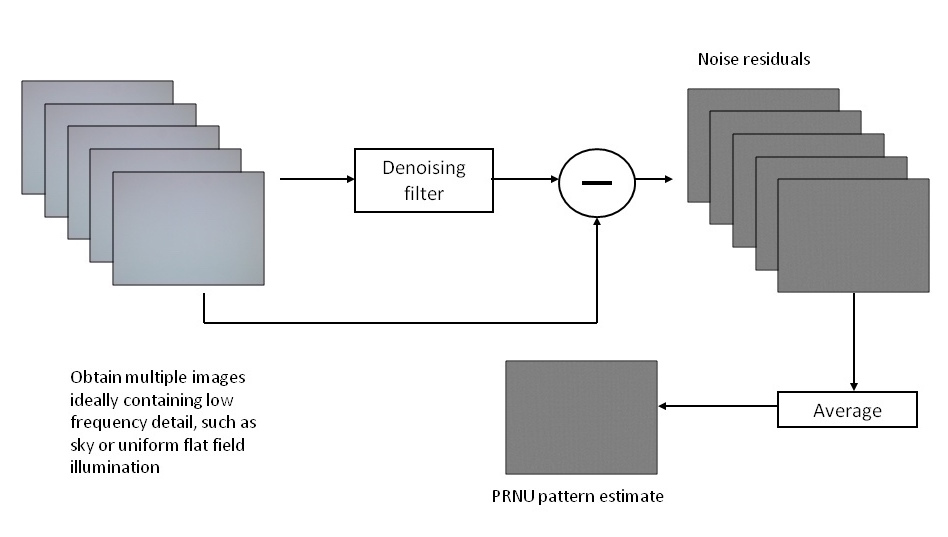
\includegraphics[width=0.8\textwidth]{../images/prnu_extraction_2}
\end{center}
  \caption{Estrazione della \emph{fingerprint} da ciascun cluster ottenuto}
\label{fig:soglia AC}
\end{figure}
\end{tframe}
\section{Validazione}
\section{Esperimenti}

\subsection{Dataset}

Per gli esperimenti è stato utilizzato un dataset che contiene un totale di 14 dispositivi, che includono smartphone e tablet, di diverse case produttrici e modelli. In particolare i modelli in nostro possesso sono: un Galaxy S3, due Galaxy S3 mini, un Galaxy S4 mini, un Galaxy Tab 3, un Galaxy Tab, un Galaxy Trend Plus, un Huawei G6, un Ipad 2, un Ipad mini, un Iphone 4S, un Iphone 5C, un Iphone 5 e un Iphone 6. Di tutti questi dispositivi siamo in possesso di immagini direttamente acquisite (immagini naturali) e delle stesse immagini ma caricate e scaricate da Facebook, in particolare ci siamo concentrati sulle immagini scaricate da Facebook in alta risoluzione.

La fase di estrazione delle fingerprint è stata eseguita tre volte con tre diversi sottoinsieme del dataset di dimensione differente. In particolare, seguendo gli esperimenti di [cit] sono stati usati insiemi da 6 dispositivi (un Galaxy S3, due Galaxy S3 mini, un Galaxy S4 mini, un Galaxy Tab 3, un Galaxy Tab), 5 dispositivi (un Huawei G6, un Ipad 2, un Ipad mini, un Iphone 4S, un Iphone 5C) e 4 dispositivi (un Galaxy Tab 3, un Galaxy Tab, un Galaxy Trend Plus, un Huawei G6). Dai dispositivi sono state selezionate 50 immagini, per un totale di 300, 250, 200 immagini rispettivamente per i tre casi.

Come spiegato in precedenza, la fase di validazione consiste nel verificare se sono state calcolate delle buone fingerprint, ovvero che siano in grado, data una generica immagine appartente al dataset non usata in precedenza, di assegnarle il giusto dispositivo. In questa fase le camere sono state suddivise in gruppi uguali alla fase di estrazione delle fingerprint, utilizzando però 20 immagini da ciascun dispositivo non usate nella fase precedente.

\subsection{Risultati}

I risultati sono molto diversi per il caso delle immagini naturali e per il caso delle immagini di Facebook in alta risoluzione. Tali risultati sono ottenuti utilizzando le modalità descritte in precedenza, ovvero Normalized Cuts con $Ncuts$ come condizione di stop con soglia pari a $10^{-5}$.

\begin{figure}[h]
\begin{center}
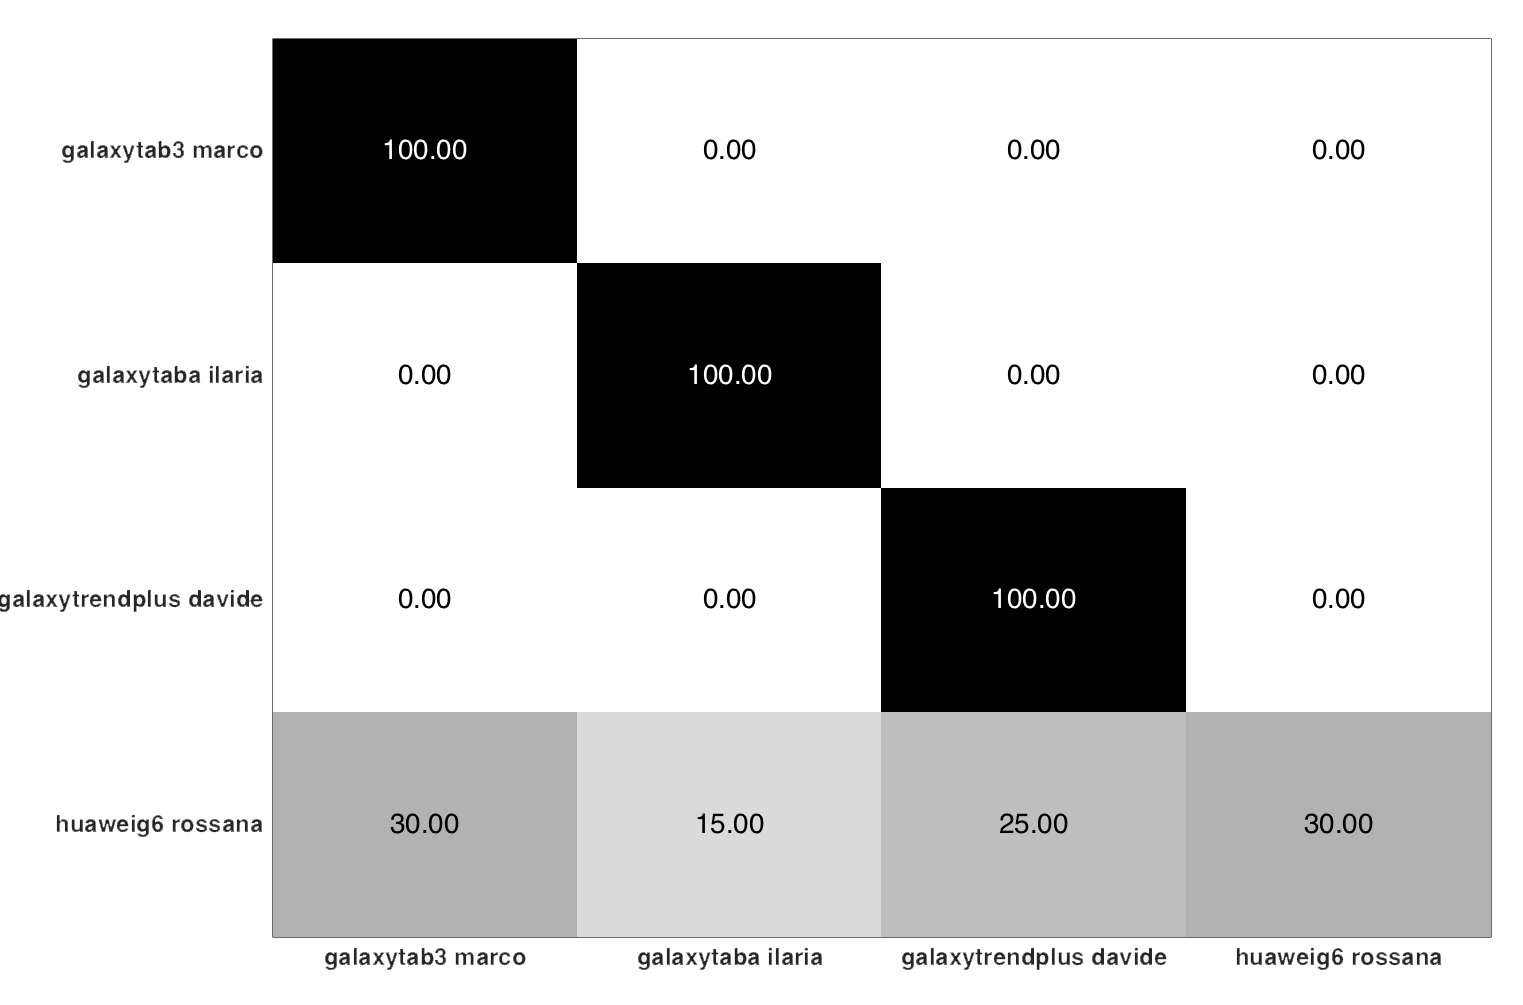
\includegraphics[width=0.4\textwidth]{images/confusionmatrix_nat_4.png}
\end{center}
  \caption{Matrice di confuzione per il caso delle immagini naturali usando 4 dispositivi.}
\label{fig:validation}
\end{figure}

\begin{figure}[h]
\begin{center}
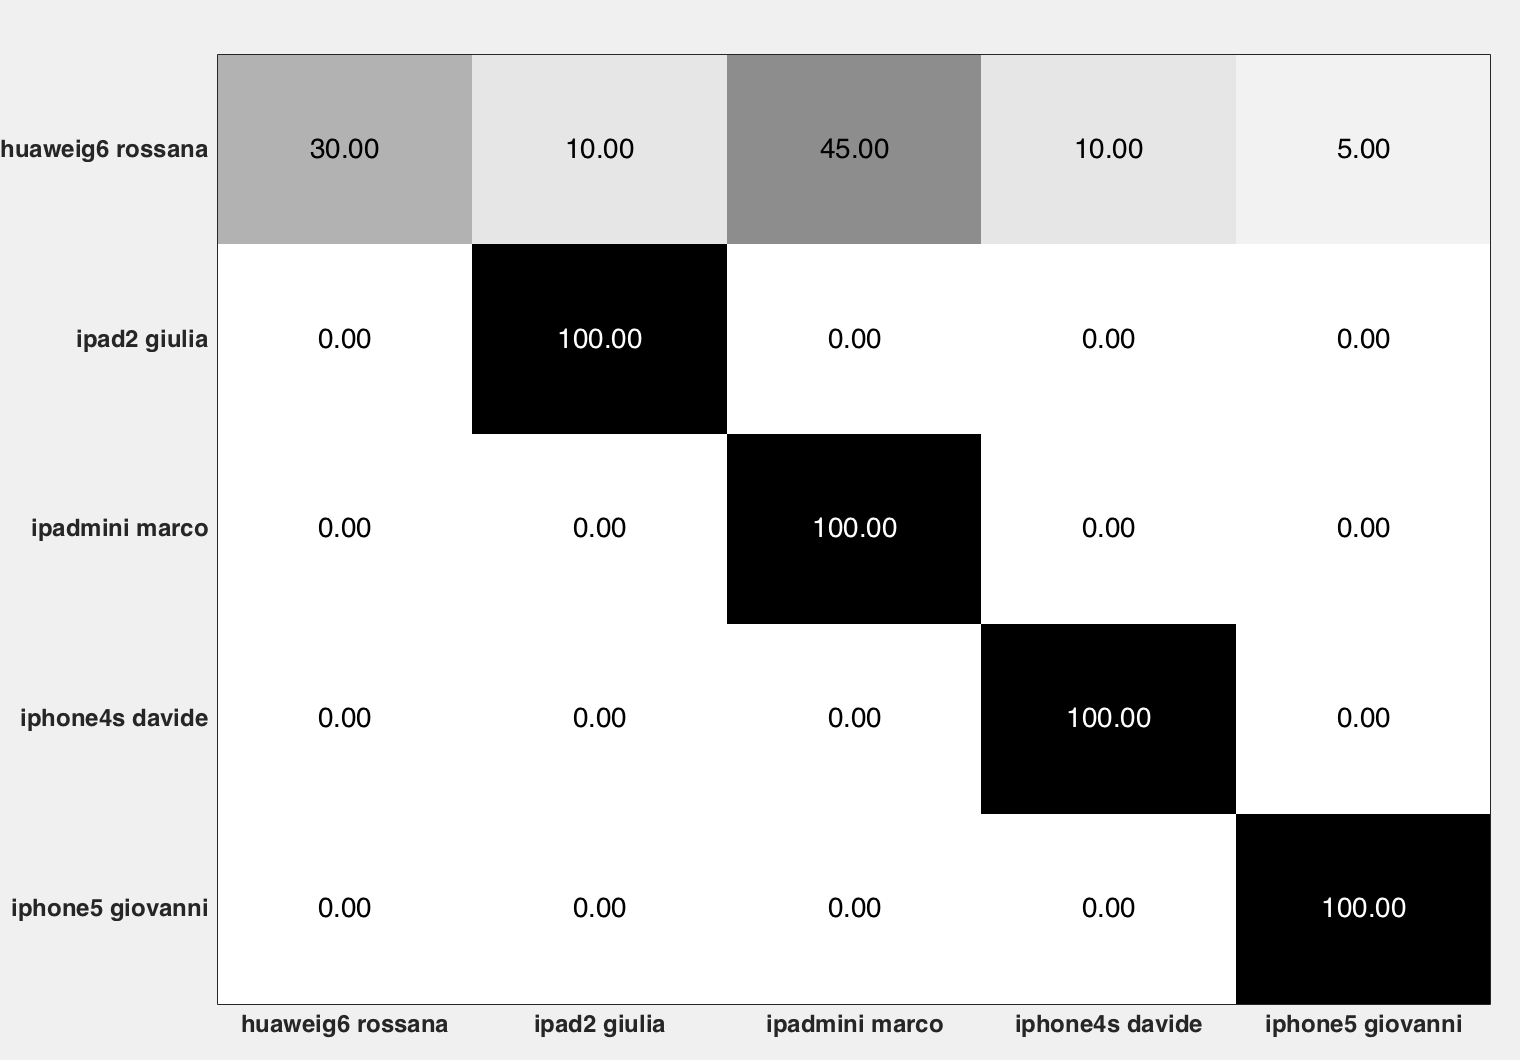
\includegraphics[width=0.4\textwidth]{images/confusionmatrix_nat_5.png}
\end{center}
  \caption{Matrice di confuzione per il caso delle immagini naturali usando 5 dispositivi.}
\label{fig:validation}
\end{figure}

\begin{figure}[h]
\begin{center}
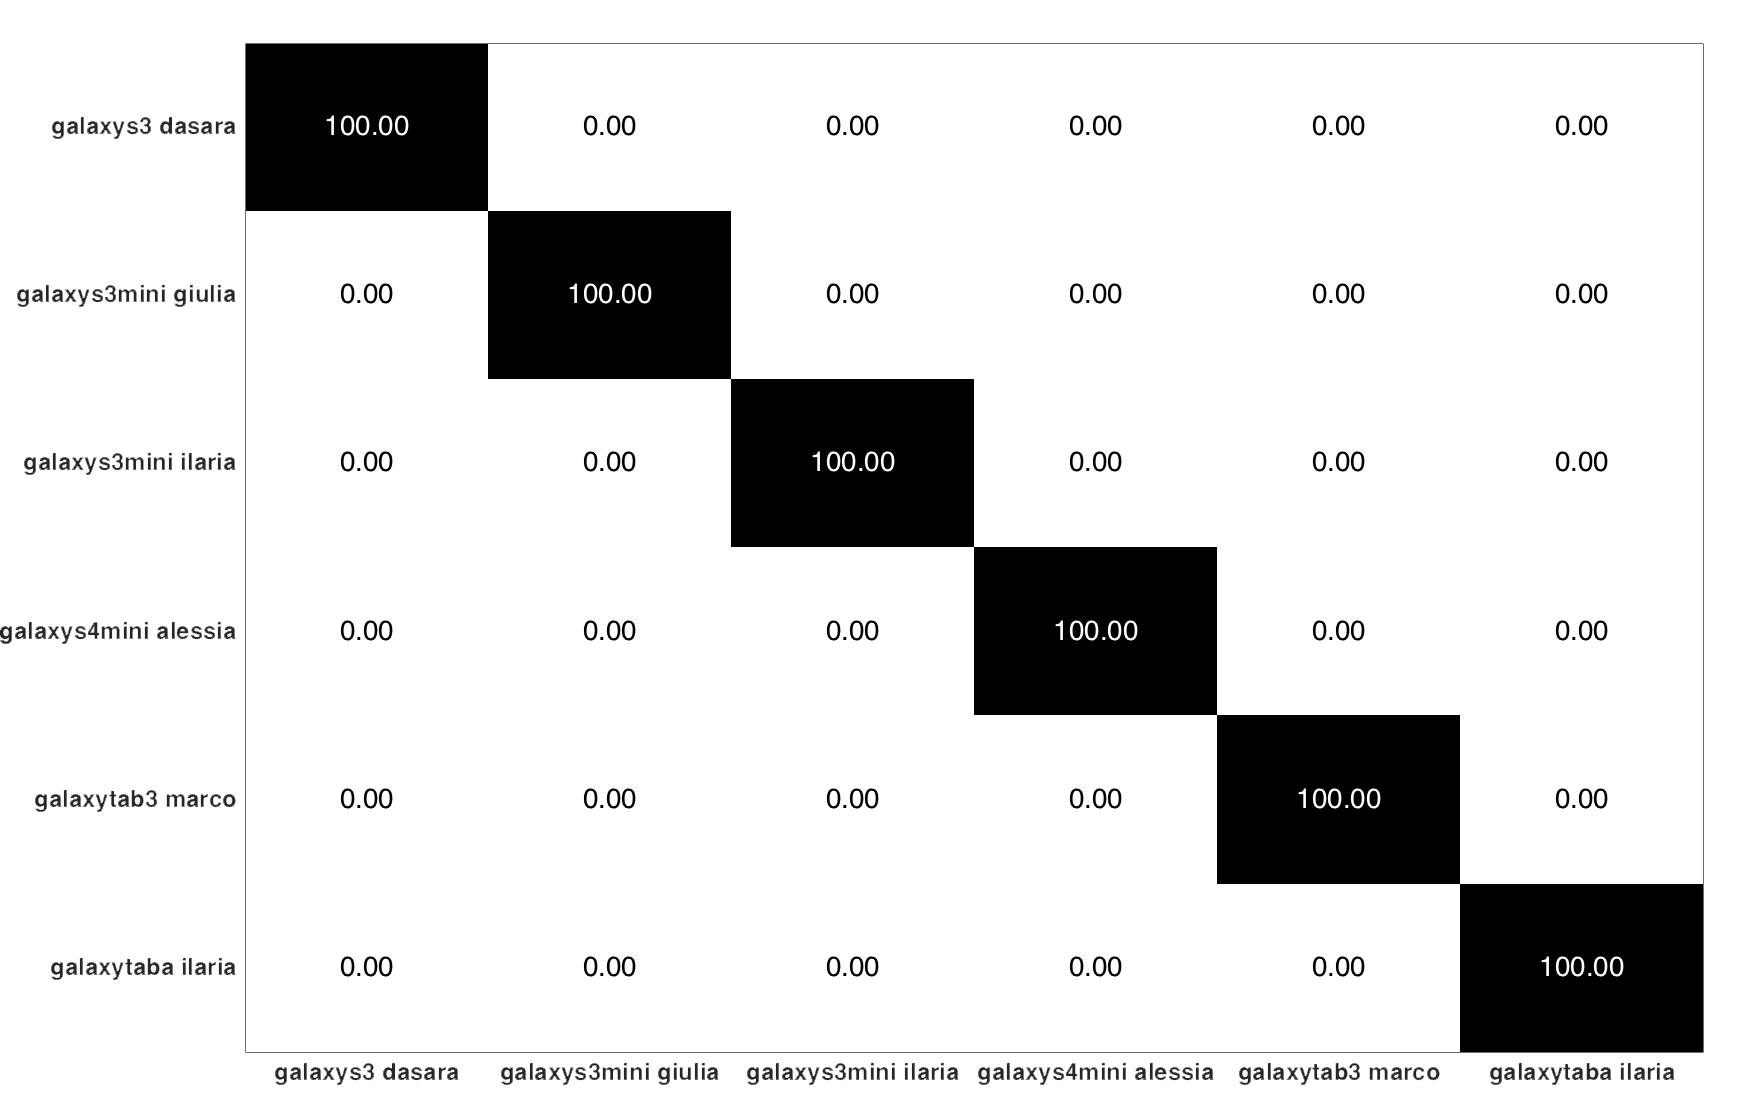
\includegraphics[width=0.4\textwidth]{images/confusionmatrix_nat_6.png}
\end{center}
  \caption{Matrice di confuzione per il caso delle immagini naturali usando 6 dispositivi.}
\label{fig:validation}
\end{figure}

Nel caso delle immagini naturali la validazione ottiene dei buoni risultati rispetto a tutte e tre le ripartizioni del dataset. Le immagini di validazione vengono associate alla giusta fingerprint con un'accuratezza del 100\% su tutti i dispositivi; l'unica eccezione è rappresentata dal dispositivo Huawei G6. Gli errori in questo caso non sono però dovuti ad una fingerprint rumorosa, poichè nella fase di clustering è stata ottenuta una percentuale di falsi positivi pari a 0. L'errore di classificazione è quindi dovuto in fase di validazione, ovvero quando, utilizzando la PCE viene calcolata la similitudine fra le immagini di test e le fingerprint estratte.

\begin{figure}[h]
\begin{center}
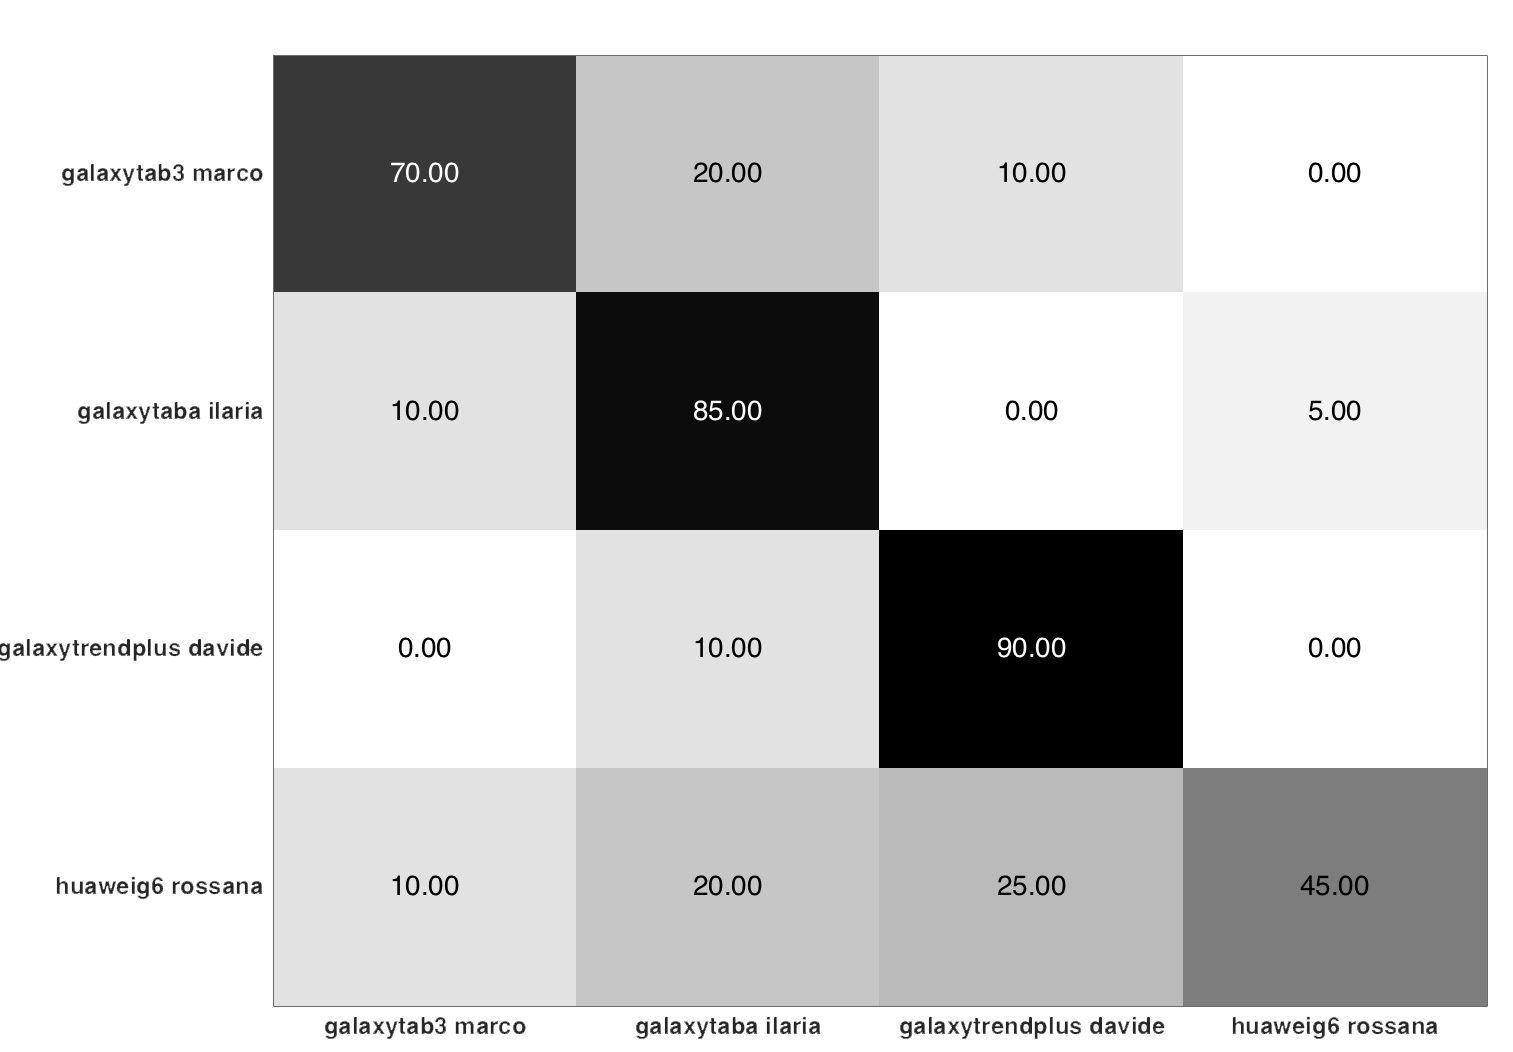
\includegraphics[width=0.4\textwidth]{images/confusionmatrix_fb_4.png}
\end{center}
  \caption{Matrice di confuzione per il caso delle immagini scaricati da Facebook usando 4 dispositivi.}
\label{fig:validation}
\end{figure}

\begin{figure}[h]
\begin{center}
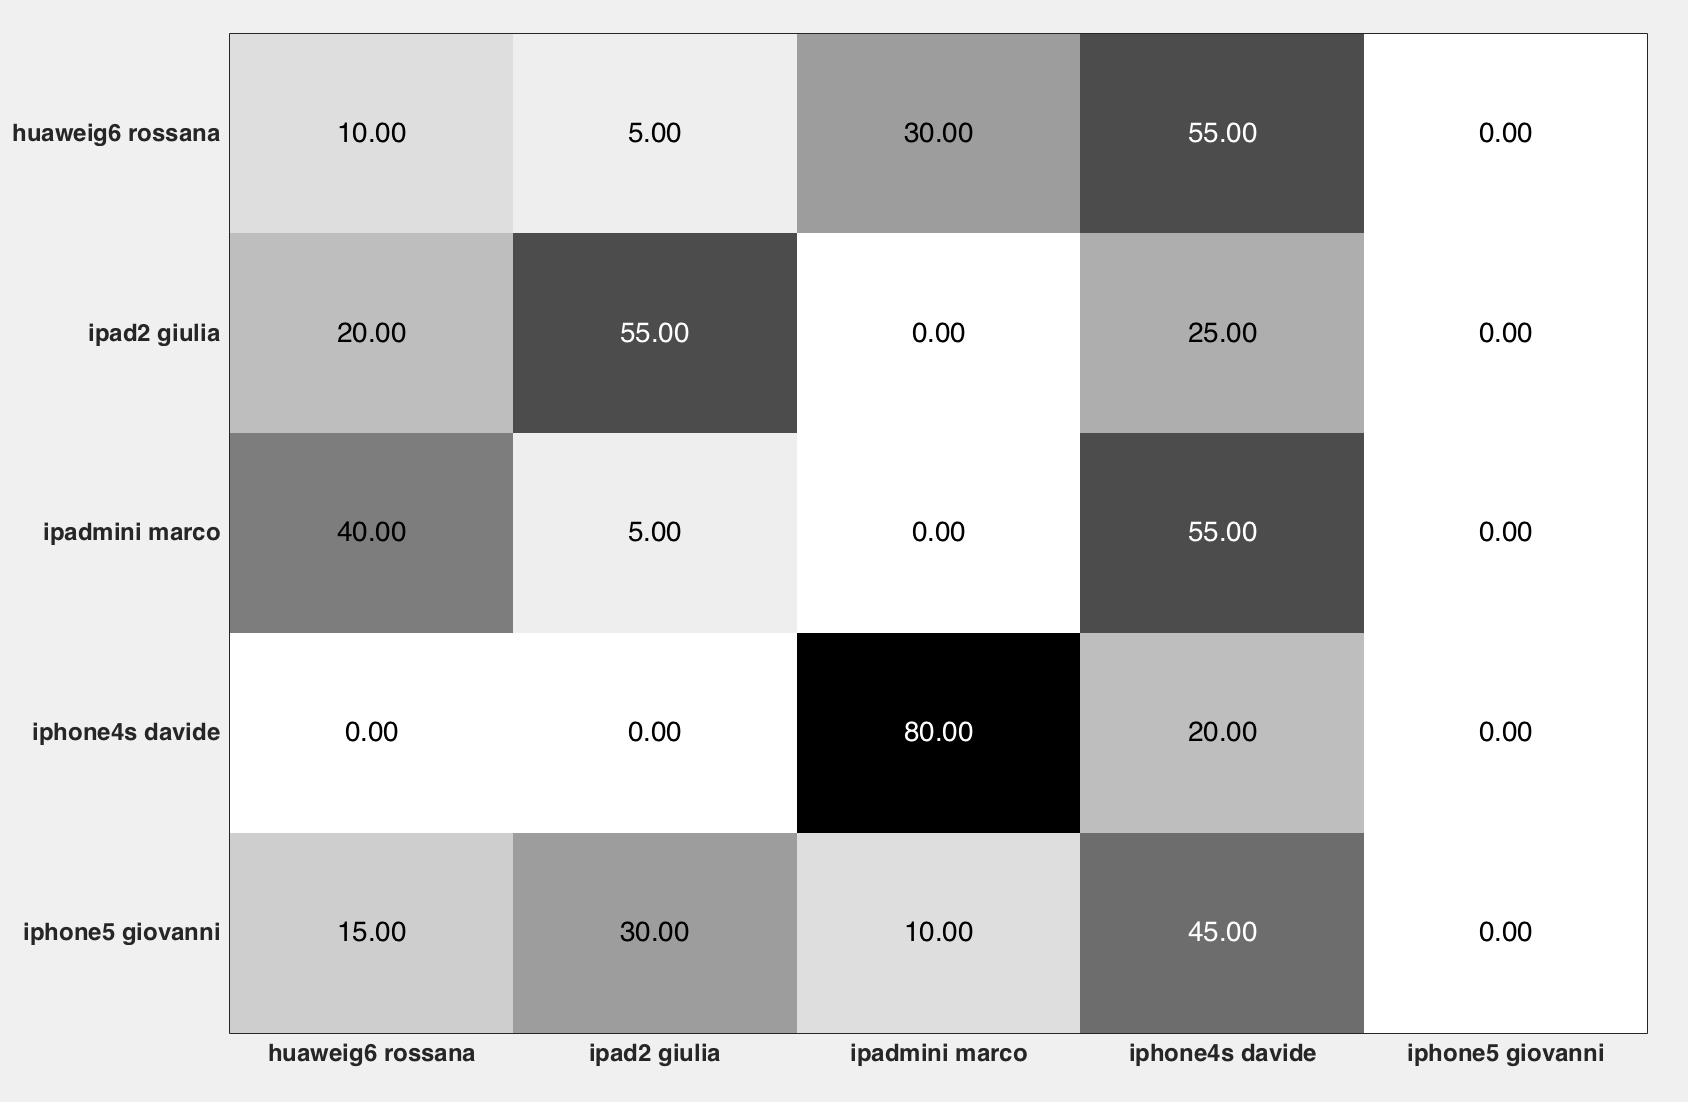
\includegraphics[width=0.4\textwidth]{images/confusionmatrix_fb_5.png}
\end{center}
  \caption{Matrice di confuzione per il caso delle immagini scaricati da Facebook usando 5 dispositivi.}
\label{fig:validation}
\end{figure}

\begin{figure}[h]
\begin{center}
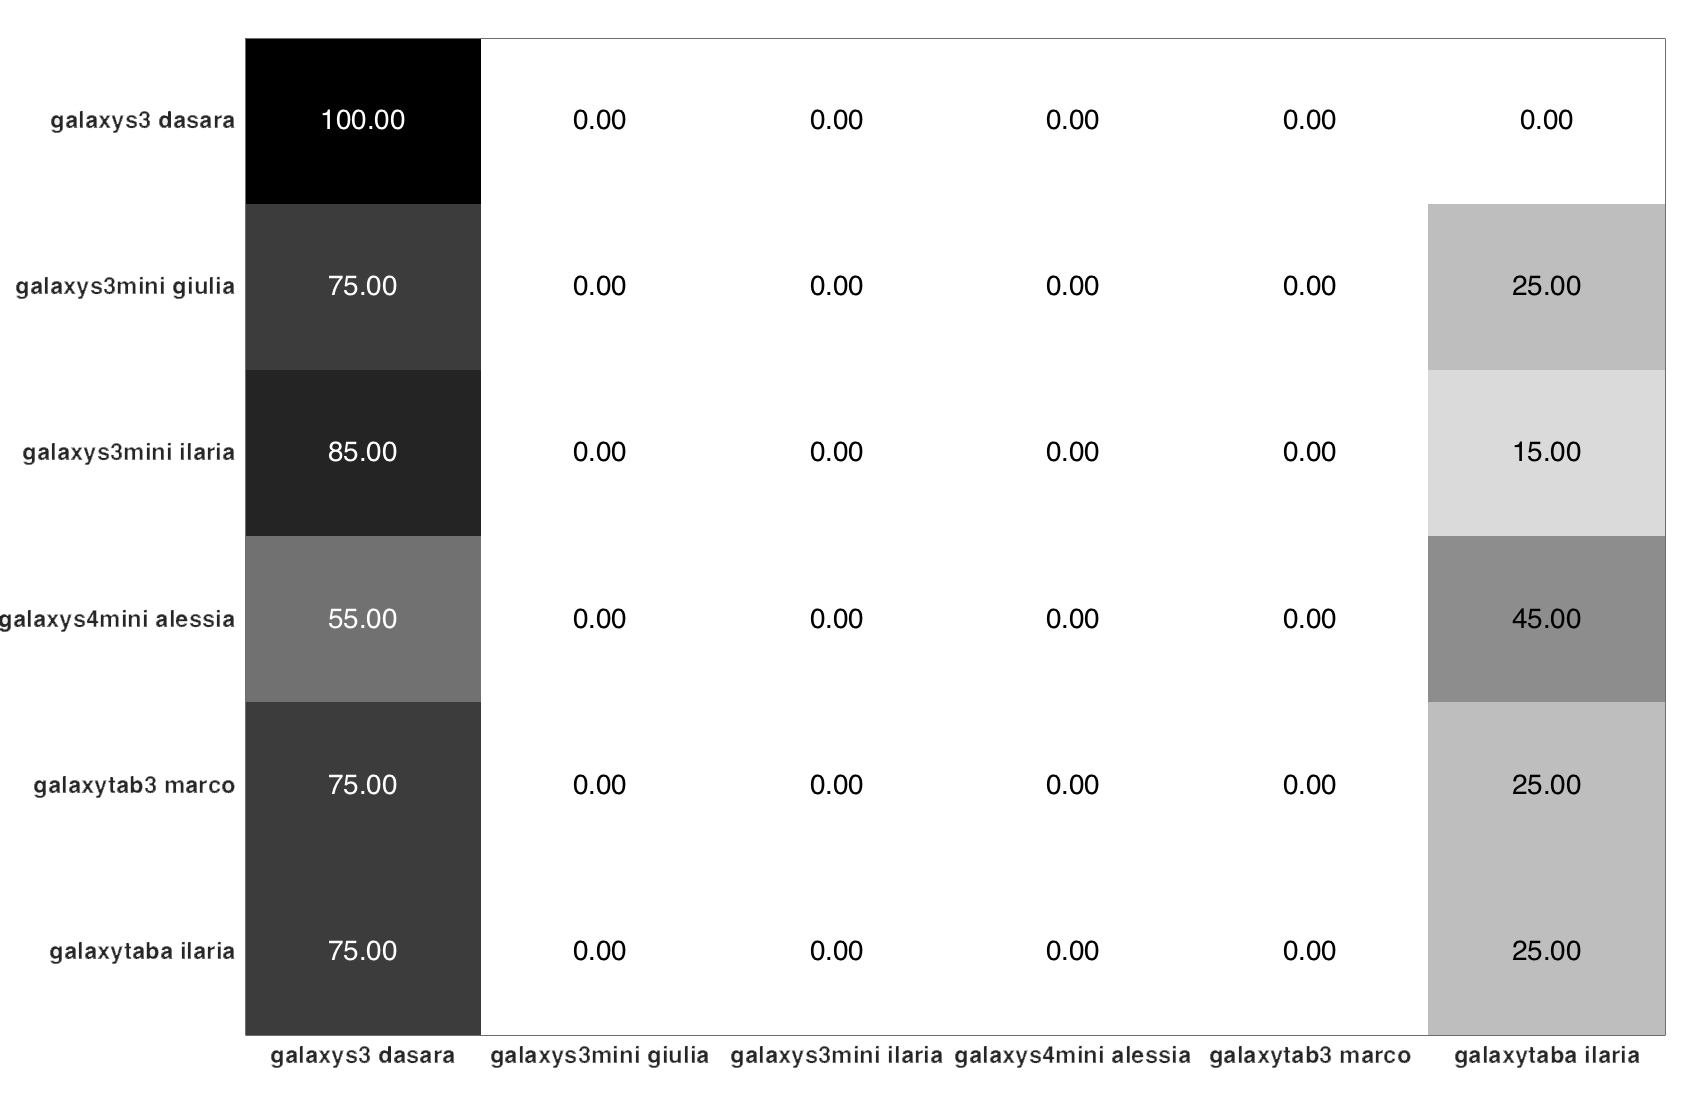
\includegraphics[width=0.4\textwidth]{images/confusionmatrix_fb_6.png}
\end{center}
  \caption{Matrice di confuzione per il caso delle immagini scaricati da Facebook usando 6 dispositivi.}
\label{fig:validation}
\end{figure}

Nel caso delle immagini scaricate da Facebook, i risultati sono inconcludenti. Solo l'insieme da 4 dispositivi, sempre ad eccezione del dispositivo Huawei G6, presenta valori accettabili. A differenza del precedente, in questo caso i molteplici errori di classificazione sono dovuti alla fase di clustering. Come mostrato nella sezione sulla selezione della soglie per il clustering, è difficile trovare una soglia che produca una clusterizzazione corretta e priva di falsi positivi, cosa che incide sulla qualità delle fingerprint. Inoltre, essendo tali immagini compresse rispetto a quelle naturali, queste perdono in informazione e così la PNRU estratta è meno significativa. Infatti i valori medi della matrice dei pesi, calcolati con la PCE,  in questo caso sono all'incirca di un ordine di grandezza inferiore rispetto ai valori medi della matrice dei pesi del caso delle immagini naturali. Ciò si ripercuote sulla soluzione dell'equazione che Normalized Cuts utilizza per partizionare il grafo.

Si può dedurre dai risultati che il nostro metodo di identificazione automatica dei dispositivi non è efficace per immagini che hanno subito una compressione, poichè le PNRU non sono sufficientemente discriminanti. Per quanto riguarda le immagini naturali, i risultati della validazione sono multo buoni ad eccezione di un unico dispositivo.
\section{Conclusioni}

In questo articolo abbiamo presentato un metodo di identificazione automatica di dispositivi a partire da un insieme di immagini la cui provenienza è ignota. Il metodo, prendendo le basi da \cite{ Amerini2014831} e apportandone alcune modifiche, funziona come segue:
\begin{enumerate}
\item Le PRNU vengono estratte dalle immagini del dataset. 
\item Per ogni coppia di PRNU viene calcolata una misura di similarità utilizzando la PCE e viene costruita una matrice dei pesi che rappresenta il grafo completamente connesso.
\item L'algoritmo Normalized Cuts partiziona il grafo e divide le immagini in clusters.
\item Per ogni clusters viene calcolata una fingerprint che rappresenta un dispositivo, a partire dalle PRNU delle immagini appartenenti a tale cluster.
\item Infine una fase di validazione che verifica la qualità delle fingerprint estratte.
\end{enumerate}

Il dataset utilizzato contiene immagini direttamente acquisite dai dispositivi e le stesse immagini caricate e poi scaricate da Facebook. I risultati ottenuti nella fase di validazione differiscono a seconda del tipo di immagini utilizzate. Le fingerprints estratte per il caso delle immagini naturali sono di qualità ed il metodo è in grado di associare una generica immagine del dataset alla fingerprint corretta, ad eccezione per le immagini provenienti dal dispositivo Huawei.

Per quanto riguarda le immagini scaricate da Facebook, il metodo si è mostrato meno efficace. Questo è dovuto alla fatto che le immagini caricate su un social network subiscono, in genere, una compressione che va peggiorare la qualità delle PRNU estratte. Questo ha conseguenze sulla misura di similarità, in questo caso la PCE. La similarità fra immagini provenienti dallo stesso dispositivo risulta meno forte rispetto a considerare la similarità delle stesse immagini per il caso delle immagini naturali. Inoltre a causa di ciò, la fase di clustering produce un numero maggior di clusters che, seppur puliti, conterranno un numero minore di immagini rispetto al caso delle immagini naturali, a causa di una TPR molto più bassa; tutto ciò va ad influire sulla qualità delle fingerprints nella fase di validazione. Va notato comunque, che la compressione, perlomeno quella effettuata da Facebook, sembra incidere maggiormente su alcuni dispositivi piuttosto che su altri, con alcuni di questi che infatti ottengono un'accuratezza nella predizione alta indipendentemente dalla ripartizione del dataset in cui si ritrovano, come mostrato nelle matrici di confusione dei vari esperimenti.

In conclusione, il metodo implementato funziona correttamente quando si estraggono delle PRNU di qualità dalle immagini, ovvero pulite e calcolate con tante immagini, cosa meno possibile se l'immagine è stata sottoposta ad una pesante compressione.

\end{document}